\chapter{部分可见积木世界构建方法}
\label{dataset}
本章旨在提出一种部分可见积木世界的构建方法,以便能够临机生成可控空间关系的部分可见积木世界图像,并生成
部分可见积木世界数据集POVQAD以便在后续研究中评估本文提出的神经符号VQA框架的性能。
下面本章将从部分可见积木世界构建任务说明、基于ASP的部分可见积木世界构建方法、POVQAD数据集的构建这三方面展开。
\section{部分可见积木世界构建任务说明}
部分可见积木世界的构建任务包括两方面:根据用户发出的自然语言的积木世界生成指令临机生成部分可见积木世界图像,以及
构建积木世界部分可见空间推理数据集POVQAD。
根据自然语言的积木世界生成指令临机生成部分可见积木世界图像对自动规矩课程的教学具有极大实际应用价值。
积木世界作为自动规划领域研究、教学的经典场景,在自动规划课程的教学实践中,教师通常需要通过控制积木之间的空间关系,
生成具有多样初始状态的任务场景,从而用于测试和演示不同规划算法在特定任务中的适用性与效果。基于这一实际需要,
需要自动规划教学系统能够做到根据用户输入的自然语言描述,实时生成满足语义约束的积木世界图像,并能够围绕该图像进行空间关系相关的视觉问答。
显然,构建符合约束的积木世界图像成为了推动自动规划课程教学进一步发展的先决条件。
而构建积木世界部分可见空间推理数据集POVQAD,则源于现有的模拟积木世界VQA的CLEVR数据集的几点缺陷:
\begin{enumerate}[nosep]
\item CLEVR中场景信息完全可见。对CLEVR中的某个问题而言,问题中涉及的所有物体,均在该问题对应的图像中
直接可见,不能反映现实世界中的部分场景可见的情形,不能满足本文研究目标中对于部分可见积木世界场景的需要。
例如,对于问题“What color is the cylinder to the left of the red sphere?”,
该问题对应的图像中左侧有一个蓝色圆柱体,右侧是红色球体。模型只需定位球体,并找其左侧物体,即可直接读取颜色。
\item CLEVR缺少环境级逻辑约束。CLEVR 场景中不存在“必须满足”的环境约束,
例如“所有红色物体必须是立方体”这类限制,使得推理任务缺乏积木世界空间推理中复杂性的模拟,不能考察模型综合利用背景知识进行系统推理的能力。
例如,对于问题“Are there more cubes than red things?”,
模型只需清点图像中立方体的数量和红色物体的数量即可比较并得出答案,而无需理解任何隐藏的逻辑条件或跨区域限制。
\item CLEVR中不存在空间推理问题。CLEVR中,空间关系只用于建立起两个或多个物体之间的联系,以便根据参照物体找到
目标物体,但是并不存在直接提问物体所在位置、物体间位置关系等等,不存在空间推理问题。
\end{enumerate}

下面本节将介绍部分可见积木世界的一些基本设定,以便为后续进行基于ASP的部分可见积木世界构建和POVQAD数据集构建奠定基础。
\subsection{部分可见积木世界的定义}
积木世界是一种被广泛应用于自动规划研究与教学的典型仿真环境,其核心特征是:由多个形状、颜色、大小各异的物体构成,
这些物体以离散方式摆放在三维空间内,并满足一定的空间布局规则。该世界的状态通常具有良好的结构性与可控性,便于形式逻辑建模与基于规则的推理。

下面本节从积木世界的基本组成、约束模板两方面对部分可见积木世界的定义展开介绍。
\subsubsection{积木世界基本组成}
积木世界的基本组成可以从以下三个主要维度进行描述:
\begin{enumerate}[nosep]
\item 物体属性。每一个积木被视为一个具备静态属性的独立个体,其属性包括以下四种:
\begin{enumerate}[nosep]
\item 形状:包括立方体、球体、圆柱体和圆锥体。
\item 颜色:红色、蓝色、绿色、黄色、灰色、棕色、紫色和青色。
\item 尺寸:小、中、大。
\item 材质:橡胶和金属。
\end{enumerate}
选取这四种基本属性,是因为它们是物体最直观且容易区分的特征,并且与原始 CLEVR 数据集保持一致,便于进行比较研究。对
每个属性的可能取值进行了限制(例如,八种颜色,四种形状,两种材质,三种尺寸),
这样做的目的是为了简化推理过程并控制答案的搜索空间,避免由于可能的属性组合过多而导致的推理复杂度过高。
\item 空间关系。本文对图像中物体之间的空间关系,选取了上、下、前、后、左、右这六种基本方向关系作为研究对象,这一设计具有以下几点合理性:
\begin{enumerate}[nosep]
\item 语义基础性强,覆盖主流空间语言表达。
这六个方向关系与人类空间认知中的基本坐标轴(x、y、z)紧密对应,构成了绝大多数空间描述中的基础语义单元。
它们不仅是自然语言中空间关系的核心词汇(如“在左边的红色球体”),也是几何推理中最基本的参照方向。
通过组合这六种关系,可以表达复杂位置结构而无需引入冗余关系。
\item 结构可控性强,便于形式化建模与推理。
选择有限的六类方向关系,有助于控制逻辑建模复杂度,避免因冗余或模糊的空间词(如“斜对角”“近旁”)引入不确定性。
每种关系均可通过规则明确定义(例如通过坐标或投影判断),适配ASP规则系统,保证推理结果的一致性和可验证性。
\item 支持三维推理,满足立体场景建模需要。
相较于只在二维平面上定义“上下左右”,引入“前后”关系使模型具备三维推理能力,更贴合真实或拟真场景下的空间认知需求。
尤其在积木堆叠或遮挡问题中,前后关系对于判断可见性与空间遮挡至关重要。
\end{enumerate}
\item 区域划分。本文对图像中的空间进行划分,形成四个区域,区域编号取值分别为0、1、2、3,并同时规定每个物体只能在图像的一个区域中,不能同时跨多个区域。
为图像空间划分区域,主要的优势在于为图像生成和问题生成指定作用范围约束,有利于提升数据集的复杂性和多样性。
\end{enumerate}
\subsubsection{部分可见性的定义}
在VQA领域,部分可见性指的是在观察场景时,图像中的部分信息由于遮挡、视角限制或场景复杂性而不可直接获得的情况。
与理想的全可见环境相比,部分可见性更符合真实世界的感知条件,也对模型的空间推理与信息补全能力提出了更高要求。
近年来,越来越多研究关注如何在部分可见的场景下完成问答任务,以增强模型在实际应用中的鲁棒性与泛化能力。

在本文所构建的积木世界场景中,我们将部分可见性进一步细分为两种典型情形,即“背景知识可推理的完全不可见”和“无需标注即可推理的部分遮挡”,
分别对应视觉遮挡的不同程度:

部分遮挡图像是“背景知识不足,且图像中被部分遮挡”的情形,这种情形代表了多数实际视觉任务中遇到的问题:
视觉系统可以检测部分被遮挡的物体,但缺乏对完整结构的观测,
难以仅靠视觉识别完成推理任务。本研究设计此类情境,旨在展示无需额外标注或监督,仅通过空间逻辑推理即可提升问答系统表现。例如:
\begin{enumerate}[nosep]
\item \textbf{图像内容(以文字描述)}:图中左侧有两个物体,其中一个绿色球体部分被另一个物体挡住,仅露出顶端。
\item \textbf{问题示例}:这个绿色球体是否位于红色立方体的上方?
\end{enumerate}
该情形下,仅凭部分视觉输入无法精确回答问题,但结合已有空间规则与遮挡顺序,系统可准确判断相对位置关系。
这类问题强调了空间逻辑推理在提升弱监督视觉问答中的作用。

全遮挡图像属于“背景知识中已知,但图像中不可见”的情形。此类情形中,某些物体或其属性未出现在图像中,但依据环境布置的规则或先验知识,推理系统应当具备“补全”或“外推”能力。
例如:
\begin{enumerate}[nosep]
\item \textbf{背景约束}:场景中所有蓝色球体都放置在红色立方体后面,且每个红色立方体后面恰好有一个蓝球。
\item \textbf{图像内容(以文字描述)}:图中可见两个红色立方体,但它们后方区域被完全遮挡。
\item \textbf{问题示例}:这个场景中是否存在蓝色球体?
\end{enumerate}
尽管视觉输入中没有检测到任何蓝球,但根据背景规则和红立方体的数量,
系统应能得出“存在两个蓝球”的结论。这类问题强调的是利用背景知识进行结构性空间推理。

在具体实现上,本文使用遮挡面积占比和遮挡关系来控制这些遮挡情形的生成。
\subsection{约束模板}
约束模板是指使用逻辑表示语言(如 ASP)抽象定义的一类通用规则形式,这些规则可以通过填入特定参数(例如区域、属性、属性值、数量等)
来实例化为具体约束,从而用于生成符合特定空间关系、区域分布或者属性限制的积木世界图像。

将约束模板引入临机生成可控空间关系的部分可见积木世界的构建中,出于以下几方面的考量:
\begin{enumerate}[nosep]
\item 保证场景的逻辑一致性。约束模板在构造场景时充当“规则”,确保生成的每个场景都遵循设定的逻辑和规律,
例如“一个区域不能有超过 3 个大物体”或“同一区域中不允许出现两个相同材质的物体”。这有助于构建符合特定认知与推理需求的合理场景。
\item 可复用、结构清晰、易于扩展。模板化的设计使得规则可以模块化、参数化、重复使用,便于添加新规则或调整已有规则。
例如要增加“区域之间不能有相同材质的物体”,只需添加一条模板,不需要重写整个生成逻辑。
\item 支撑任务复杂度的调控。通过对模板赋予不同的参数,生成不同的约束,以及约束之间的各种组合,可以人为控制
任务难度和积木世界的复杂度。
\item 提升部分可见积木世界的多样性和可控性。通过预先设计一系列模板,可以系统地控制场景多样性
(如属性组合、空间关系、数量限制)而不是随机生成。这种可控性有助于评估模型对不同类型推理问题的能力。
\end{enumerate}

在约束模板的设计上,本文针对部分遮挡和完全遮挡两种情况,设计了约束模板,并以ASP形式给出。
使用ASP来进行表示的原因在于,ASP 是一种声明式逻辑编程语言,特别擅长用于描述约束、规则、组合问题,通过使用 ASP,可以形式化地定义物体属性、数量、空间关系等复杂逻辑要求。
以下为部分约束模板示例,所有的约束模板在附录\ref{appendix:constraints}中予以展示。
\begin{enumerate}[nosep]
\item 遮挡关系的物体对数不少于N。
\begin{lstlisting}
:- #count{X,Y : occludes(X,Y), obj(X), obj(Y)} < N.
\end{lstlisting}
\item 每个被遮挡物体的遮挡率不超过R'。
\begin{lstlisting}
:- occlusion_rate(T, R0), R0 > R_prime.
\end{lstlisting}
\item 区域R中的物体最多有N个。
\begin{lstlisting}
:- #count{X: obj(X), at(X,R)} > N.
\end{lstlisting}
\item 场景中至少有K对物体呈现“左-右”相邻的空间关系。
\begin{lstlisting}
:- #count{X,Y: left(X,Y), obj(X), obj(Y)} < K.
\end{lstlisting}
\item 目标物体的左侧有且只有L个物体。
\begin{lstlisting}
:- #count{X: left(X,T), obj(X)} != L.
\end{lstlisting}
\end{enumerate}
\subsection{根据约束构建部分可见积木世界}
获得约束规则后,仍需要进行一系列流程方能获得部分可见积木世界图像。下面在此对后续流程进行简要介绍,具体的实现细节因构建任务
的不同而略有差异,将分别在3.2节基于ASP的部分可见积木世界的构建和3.3节POVQAD数据集构建中分别予以介绍。
\begin{enumerate}[nosep]
\item 生成环境。在获得具体约束规则之后,需要进一步生成环境。
环境是根据若干条约束规则生成的,表示部分可见积木世界必须遵守的一系列限制条件。
在具体流程上,需要将全局约束与获得的具体约束规则进行组合,共同输入ASP求解器进行求解。若能正常执行并获得至少一个答案集,
则表明获得的具体约束规则之间没有出现逻辑冲突的情况,可以获得环境,后续可以据此生成部分可见积木世界图像。若执行报错或者答案集为空,
则表明不能获得环境,停止进行后续进一步的流程。全局约束是所有环境都应遵循的约束,对整个积木世界进行了基本定义,
例如“平面区域划分为4个,编号0、1、2、3。”就是通过全局约束定义的,
ASP形式为\texttt{region(0). region(1). region(2). region(3).}。
本文所用的所有全局约束在附录\ref{appendix:environment}予以了展示。
\item 构建场景。场景是一个具体的实例化结果,描述了一个满足环境的要求的积木世界布局,包括了积木世界中所有对象的属性、
位置及其相互空间关系、图像等等。场景是环境的具体化,与图像和关于图像的问题生成直接相关。在生成场景的过程中,需要依据完整场景图进行进一步的生成。
完整场景图中包括了所有对象的属性。

构建场景的大致流程如下:首先将环境输入ASP求解器进行求解,获得满足环境的答案集,此处一个答案集对应一个完整场景图。
随后,根据实际需要,生成部分可见场景图(部分遮挡的情形)和不可见场景图(完全遮挡的情形),以供后续生成图像使用。
部分可见场景图和不可见场景图分别对应部分可见场景和不可见场景,此时已经基本完成两种场景的生成,但仍缺少图像信息,需要
生成图像环节进行进一步的处理。
\item 生成图像。基于部分可见场景图和不可见场景图,使用Blender进行渲染生成图像,并完善前一步中生成的基本完整的场景,获得最终的
部分可见场景和不可见场景。
\end{enumerate}

本章后续的基于ASP的部分可见积木世界的构建和POVQAD数据集构建,都将大致按照上述流程进行,最终获得部分可见积木世界的图像。
\section{基于ASP的部分可见积木世界构建方法}
\subsection{构建目标与技术选型}
构建基于ASP的部分可见积木世界的总目标为:LLM能够根据用户提供的以自然语言形式描述的对积木世界中物体属性、遮挡关系
等方面的要求,生成具体的以ASP形式描述的约束规则,以供后续生成环境使用。基于这一总目标,本文决定采用提示学习的方法,
使用DSPy作为提示管理与语义生成框架,让LLM习得预定义的约束模板中的深层语义,使其掌握如何根据用户要求进行对应的ASP约束生成。
选择基于ASP来构建部分可见积木世界,有以下几点原因:
\begin{enumerate}[nosep]
\item ASP具有明确的逻辑语义和出色的可解释性,能够对积木世界中关于位置、遮挡、颜色、堆叠关系等复杂规则进行形式化建模,同时保证生成图像的语义一致性和规则可追溯性。
\item ASP支持非单调逻辑和默认推理,能够自然处理部分可见场景中关于不确定信息的表达,如“某个物体可能被遮挡”或“在未观察到的情况下推测其存在”,这一特性恰好契合本文数据集所需建模的现实感知不完全性。
\item ASP具备高效的求解器(如 Clingo),能够在大规模规则集合下快速生成满足约束的实例,便于数据集大批量合成。
\end{enumerate}
而选择采用对LLM进行提示学习的方法,并使用DSPy来实现提示学习,出于以下几点考量:
\begin{enumerate}[nosep]
\item LLM在经过精心设计的提示引导下,能够在无需额外训练的条件下,对自然语言进行结构化转换,自动生成语法正确且语义准确的ASP规则,从而大幅降低规则生成的门槛,实现自然语言到形式化逻辑的高效映射。
\item 提示学习方法具有更强的灵活性和泛化能力。传统的数据驱动方法往往需要大量标注好的场景-约束对以训练一个专用模型,而这在积木世界中高维组合空间下代价极高且难以穷尽所有规则变体。相比之下,提示学习方式可通过少量示例演示(in-context learning)来引导LLM快速适应特定风格的规则生成任务,有效降低训练样本依赖,提升低资源条件下的数据生成效率。
\item Dspy 支持以声明式模块化方式组织提示,通过将任务划分为结构清晰的子模块(如信息提取、格式转换、规则生成等),能够更好地管理提示的复杂性与多样性。这一特性对于本任务中“从自然语言描述到ASP规则生成”的流程尤为重要,因其涉及多个阶段的信息加工与转换过程,Dspy提供的模块组合与链式执行机制(Chain of Prompts)有助于确保生成过程的逻辑一致性和中间步骤可控性。
\item Dspy 框架原生支持 与大语言模型的集成和输出约束,包括结构化输出格式、示例演示(few-shot prompting)、多候选响应重排序(reranking)等机制。对于本任务而言,ASP规则具有严格的语法与逻辑要求,Dspy 提供的 Signature 接口允许精确定义输入-输出格式,使生成的规则更符合目标结构。同时,它还支持在候选结果中选择最优输出,提升了ASP规则生成的正确率与稳定性。
\item Dspy 支持与评估指标联动的“自我改进”机制,可在一定程度上对提示进行自动优化,从而提升生成结果质量。
\end{enumerate}

以下将对构建流程展开介绍。
\subsection{构建流程}
\subsubsection{LLM生成约束}
\begin{enumerate}[nosep]
\item 任务定义。
DSPy是一个面向语言任务的程序性提示框架,能够在具备结构化的输入输出约束的前提下,
调用LLM完成特定子任务。在本任务中,将“自然语言描述的部分可见积木世界应满足的约束规则$\rightarrow$以ASP表示的部分可见积木世界的约束规则”建模为一个标准的DSPy模块。在实现上,通过DSPy的\texttt{Signature}定义任务结构,其中明确了模块的目标,即根据用户输入的部分可见积木世界应满足的约束规则生成其对应的ASP表示。
\begin{lstlisting}
class ParseQuestionToASP(Signature):
    question = dspy.InputField(desc="自然语言描述的部分可见积木世界应满足的约束规则")
    asp_code = dspy.OutputField(desc="以ASP表示的部分可见积木世界的约束规则")
\end{lstlisting}
\item 提示词设计。
本节基于已设计的约束模板设计提示词,要求LLM学习如何根据以自然语言形式描述的部分可见积木世界限制条件
生成对应的ASP规则。以下为部分提示词的示例:
\begin{lstlisting}
下面将提供给你几组以自然语言描述的对部分可见积木世界的限制条件,以及各个限制条件对应的以ASP形式表示的约束,请你学习如何根据自然语言生成这些ASP形式的约束。
在后续的对话中,将会向你发送一系列自然语言描述,需要你分别以ASP形式进行表示。

自然语言描述:遮挡关系的物体对数不少于N。
ASP规则::- #count{X,Y : occludes(X,Y), obj(X), obj(Y)} < N.

自然语言描述:每个被遮挡物体的遮挡率不超过R'。
ASP规则::- occlusion_rate(T, R0), R0 > R_prime.

自然语言描述:区域R中的物体最多有N个。
ASP规则::- #count{X: obj(X), at(X,R)} > N.

自然语言描述:场景中至少有K对物体呈现“左-右”相邻的空间关系。
ASP规则::- #count{X,Y: left(X,Y), obj(X), obj(Y)} < K.

自然语言描述:目标物体的左侧有且只有L个物体。
ASP规则::- #count{X: left(X,T), obj(X)} != L.
\end{lstlisting}
\item 提示词优化。
为进一步提升提示学习的效果,提升生成描述部分可见积木世界的ASP约束的准确率,本文在此引入验证集驱动的提示优化策略。本文设计了另一组同类的约束模板组成验证集,通过
生成ASP约束的语法正确率和语义正确率对few-shot示例顺序与提示模板进行自动调整。
语法是否正确的判断标准是:ASP程序输入Clingo后,如果能够正常执行,不提示错误,则视为语法正确,否则视为语法错误。
语义是否正确的判断标准是:要求LLM根据验证集中以自然语言描述的对部分可见积木世界的约束,来生成对应的ASP程序。
此后将生成的ASP程序经Clingo获得的执行结果和验证集中自然语言描述对应的约束经Clingo执行的结果进行比较。
如果两者的执行结果一致,则可认为语义正确,否则认为语义错误。
此处采用 DSPy 提供的 BootstrappedFewShotOptimizer 优化器,以生成的 ASP 约束的语法正确率和语义正确率作为评价指标,训练优化提示内容。
选择 BootstrappedFewShotOptimizer 优化器主要基于以下几点考量:
\begin{enumerate}[nosep]
\item 与结构化问答任务不同,用户描述的约束常常具有多种表达方式
(如“不能出现红色球体”“区域1不应有红球”等语义等价描述)。BootstrapFewShotOptimizer 
能够通过自举式学习不断挖掘多样示例,提升提示对自然语言语义变体的适应能力。
\item 本任务的输出为 ASP 形式的逻辑规则,具备明确结构与语法约束。该优化器具备结构保持能力,
能稳定生成语法正确、模板匹配度高的 ASP 表达式,从而保证数据质量。
\item 在样本数量有限的前提下,该优化器能基于已有示例动态构造 Few-shot 提示组,降低对大规模人工标注的依赖,显著减少模板调试成本。
\item BootstrapFewShotOptimizer 支持通过自定义评估函数对生成结果进行语义检查,从而形成闭环优化机制,提升生成质量。
\item 优化后的提示不仅适用于当前任务,还可迁移到其他类似的规则抽取任务中(如空间约束生成、场景逻辑分析等),为后续研究提供通用工具基础。
\end{enumerate}
\item 输出。
经过优化后的提示模块,能够将输入的以自然语言描述的对部分可见积木世界的约束,准确地转换为ASP规则。
例如,针对输入“积木世界的所有物体之间,最多有4对‘前-后’空间关系”,LLM最终输出示例如下:
\begin{lstlisting}
:- #count{X,Y: front(X,Y), obj(X), obj(Y)} < K.
\end{lstlisting}
生成的ASP规则在后续将用于环境的生成,为部分可见积木世界数据集的生成奠定坚实基础。
\end{enumerate}
\subsubsection{生成环境}
环境是根据若干条约束规则生成的,表示部分可见积木世界必须遵守的一系列限制条件。
在基于ASP的部分可见积木世界构建中,环境即“用户以自然语言描述的生成指令在经过LLM处理后生成的基于ASP的约束规则与全局约束规则,两者
共同输入ASP求解器后所得的答案集”。

那么在生成环境时,将全局约束规则与LLM生成的约束规则进行拼接,形成完整ASP程序,并由Clingo对ASP程序进行求解。
如果Clingo的输出至少存在一个答案集,说明当前约束可满足,将所得结果(即环境)保存到ASP程序的\texttt{.lp}文件中。
如果Clingo没有答案集,说明当前约束不满足(unsatisfiable),不再继续进行部分可见积木世界的生成。
\subsubsection{构建场景}
场景是基于环境的基础上进一步生成而得。将环境的\texttt{.lp}文件输入Clingo进行求解,得到若干个答案集。
此后,对答案集进行解析,以获得完整场景图。对答案集进行解析的过程实际上是对谓词进行解析的过程,主要\texttt{has\_property}和\texttt{at}两个谓词进行解析,
最终形成以JSON格式存储的场景图。

随后,检查答案集中是否存在部分遮挡约束(以谓词\texttt{occludes}和谓词\texttt{occlusion\_rate}共同表示,且遮挡面积比例大于0小于1的情况)
、完全遮挡约束(以谓词\texttt{occludes}和谓词\texttt{occlusion\_rate}共同表示,且遮挡面积比例等于1的情况)。
如果存在,则分情况进行如下操作:
\begin{enumerate}[nosep]
\item 部分遮挡(\texttt{occlusion\_rate}中遮挡面积比例$0 < R < 1$):在原有的完整场景图的基础上,添加occlusion字段的信息,例如:
\begin{lstlisting}
{
  "occlusion": [
    {0, 1, 0.3}
  ]
}
\end{lstlisting}
occlusion字段中,每个三元组都表示一对遮挡关系。其中第一个表示被遮挡物体的编号,第二个表示遮挡物体的编号,编号均与完整场景图的objects
中的物体编号保持一致。其次,遮挡面积比例$R$作为三元组的第三个数据项。在后续Blender根据场景图渲染生成积木世界图像时,将会
将两个物体按照指定的遮挡面积比例和被遮挡关系进行生成。
\item 完全遮挡(\texttt{occlusion\_rate}中遮挡面积比例$R = 1$):在原有完整场景图的基础上,将\texttt{occludes}中的
被遮挡对象(即谓词中的第一个物体)的相关信息从完整场景图的objects字段中进行删除,以模拟完全遮挡发生时,图像中无法直接感知到任何信息的情况。
\end{enumerate}
经过以上谓词解析的过程,得到部分可见场景或者完全不可见场景,以便后续Blender进行渲染生成图像。
\subsubsection{生成图像}
生成图像的目的是:根据前一步生成的基本完整的场景中的物体信息,使用Blender进行渲染,最终生成部分可见积木世界图像。
\begin{enumerate}[nosep]
\item 初始化Blender渲染对象。在这一步中,主要是设置一系列渲染参数,包括分辨率、GPU设置等等。
\item 定义场景字典。该字典中保存了场景的元信息(即将生成的图片名称等)、物体信息和方向信息。
\item 方向向量计算。先获取在场景初始化时添加的平面的法向量,此后计算摄像机的方向向量,并将
摄像机的方向向量投影到平面上,得到相对于平面的方向向量。计算完成之后,将平面删除,避免影响后续渲染。
\item 向场景中添加物体。根据场景图中的物体信息,将物体添加到场景中。
在生成部分可见场景的图像时,要注意根据\texttt{occlusion}字段中各个三元组提供的遮挡关系,来生成遮挡的情形。
\item 计算物体之间关系。基于物体的三维坐标和场景的方向向量,遍历场景中的每对物体,
计算得出空间中上、下、左、右、前、后等关系。判断两个物体之间是否存在某种关系的阈值设置为0.2,即如果两个物体之间的
方向向量的点积大于0.2,那么认为它们具有该关系。阈值可以自定义进行修改。
\end{enumerate}

\subsection{转化正确率实验}
实验目的、实验数据集、实验方法、实验结论。
本实验的目的为:验证本文提出的基于ASP的部分可见积木世界构建方法中,LLM将自然语言的积木世界生成指令转化为对应的约束的准确率。

另外,本实验在DeepSeek-Coder、LLaMA3和ChatGPT-4o三种LLM上进行实验。

实验结果如表所示。
\subsection{效率评价实验}
本实验的目的是评估基于ASP的部分可见积木世界构建方法的执行效率,验证该方法是否能够满足自动规矩课堂教学中对生成积木世界图像的速度要求。

实验数据集仍采用。

实验结果如图\ref{}所示,在
\section{POVQAD数据集构建}
本节从数据集定义、构建过程及数据集质量评估三方面展开介绍。
\subsection{数据集定义}
基于上述构建目标,本文将POVQAD数据集形式化定义为一个五元组的集合:
$$D = \{ (I_i,P_i,Q_i,\Pi_i ,A_i) | i=1,2,...,N \}$$
其中,每个元素$(I_i,P_i,Q_i,\Pi_i ,A_i)$是数据集中的一个样例,各组成部分定义如下:
\begin{enumerate}[nosep]
\item \textbf{$I_i$}为图像,是通过 Blender 渲染的基于场景生成的 3D 图像。
每张图像表示一个三维积木世界场景,所有可见物体均按预定义属性摆放。每个图像中都刻意隐藏了一个物体或者一个物体遮挡了另一个物体的一部分,以模拟部分可见条件。
图像示例如图\ref{POVQAD-figure}。
\begin{figure}
\centering
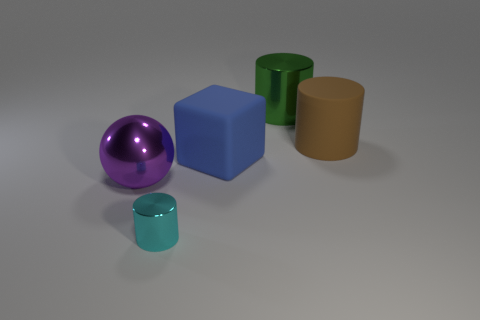
\includegraphics[scale=0.6]{figures/POVQAD中图像示例.png}
\caption{POVQAD中图像示例}
\label{POVQAD-figure}
\end{figure}
\item \textbf{$S_i$}为场景,包含了图像中的所有物体及其属性和位置关系,以JSON格式存储。
\item \textbf{$Q_i$}为问题,使用自然语言形式进行表示,例如“What shape is the small red object that is to the left of the yellow cube?”。
所有问题均为属性查询类问题,专门针对物体的四个属性之一:颜色、尺寸、形状或材质。
\item \textbf{$QA_i$}为问题的ASP表示,例如:
\begin{lstlisting}
query(Q) :-
  has_property(X, color, Q),has_property(X, shape, cylinder),
  has_property(Y, shape, sphere),has_property(Y, color, red),
  left(Y, X),same_material(X, Y),X != Y.
\end{lstlisting}
\item \textbf{$\Pi_i$}为环境,是当前图像所属的一组约束规则,采用ASP进行表示。以下为一组约束示例:
\begin{lstlisting}
% 约束示例
% 区域0中所有物体的形状必须是圆柱体
:- obj(X), at(X, 0), has_property(X, shape, cylinder).
% 区域1中蓝色物体的数量大于2个
:- #count{X: has_property(X, color, blue), at(X, 1)} > 2.
\end{lstlisting}
\item \textbf{$A_i$}为答案集,表示该问题对应的正确答案。
\end{enumerate}
\subsection{构建过程}
POVQAD的构建流程如图\ref{fig:dataset-generation}所示,共包括4个步骤。各个步骤的功能如下:
\begin{enumerate}[nosep]
\item \textbf{生成环境}:随机选取部分约束模板,并将模板实例化,最终得到环境。
\item \textbf{构建场景图}:将环境实例化,并将环境输入ASP求解器进行求解,分别生成部分可见场景图和不可见场景图。
\item \textbf{图像渲染}:使用Blender对场景图进行渲染,获得积木世界图像与场景。
\item \textbf{问题生成}:根据问题模板与场景,生成问题与其对应ASP查询,使用Clingo得到问题的答案集并对答案集进行筛选。
\end{enumerate}
\begin{figure}[h]
\centering
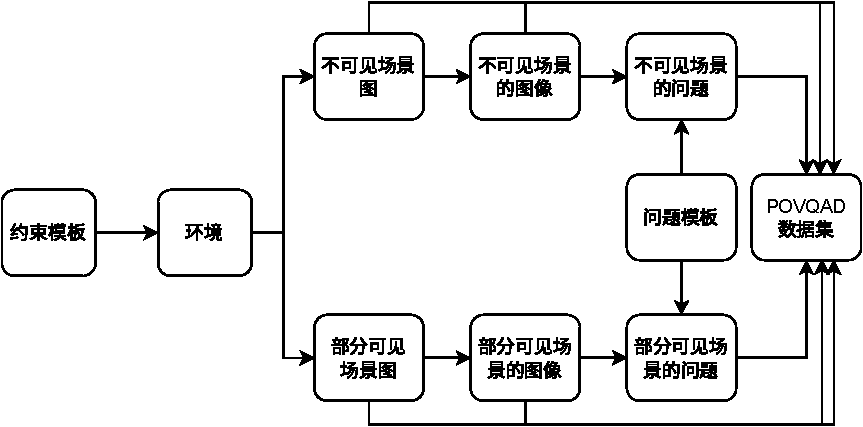
\includegraphics{figures/pipeline-POVQAD-crop.pdf}
\caption{POVQAD构建流程}
\label{fig:dataset-generation}
\end{figure}

\subsubsection{生成环境}
在POVQAD中,一个环境包含了一组约束规则,用于限定在该环境下生成的所有场景所必须满足的
属性组合、区域位置的约束条件。环境的作用是,在宏观层面上对后续生成的图像、问题进行把控,
以控制场景复杂度,并保证数据集保持逻辑一致性。在数学上可以如下表示环境:
$$ \varepsilon = \{C_1,C_2, ..., C_k \}, C_i \in ASP \quad Constraint $$
其中,每个$C_i$是用 ASP 表示的一条逻辑约束规则。

环境的生成过程包括以下步骤:(1)预定义约束模板;(2)确定模板中的相关参数;(3)对所有生成的约束经语义检查与逻辑一致性验证。

约束模板是依据常见的逻辑组合来进行设计的,覆盖了取值限定、逻辑否、逻辑或等基本逻辑模式,
部分约束模板的ASP编码表示以及对应表示含义见表\ref{tab:asp_templates},全部约束模板见附录\ref{appendix:constraints}。
除了约束模板之外,还有全局约束。
全局约束是所有生成的环境都应遵循的约束,对整个积木世界进行了基本定义,例如“平面区域划分为4个,编号0、1、2、3。”就是通过全局约束定义的,
ASP形式为\texttt{region(0). region(1). region(2). region(3).}。
本文所用的所有全局约束在附录\ref{appendix:environment}同样予以了展示。
\begin{table}[h]
    \centering
    \renewcommand{\arraystretch}{1.0}
    \begin{tabular}{|p{2.8cm}|p{12.2cm}|}
        \hline
        \textbf{模板} & \textbf{描述} \\
        \hline
        \textbf{模板1(取值约束)} & 
        \texttt{:- obj(X), at(X, R), not has\_property(X, P1, V1).} \\ 
        & 解释: 对区域R中的所有物体,它们P1属性的取值均为V1。 \\ 
        & 具体实现: :- obj(X), at(X, 0), not has\_property(X, color, red). \\
        \hline
        \textbf{模板2(遮挡比例约束)} & 
        \texttt{:- occlusion\_rate(T, R), (R <= 0; R >= 1).} \\ 
        & 解释:物体T被遮挡的比例为R(0<R<=1),完全遮挡时R=1。 \\ 
        & 具体实现::- occlusion\_rate(T, 0.1). \\
        \hline
    \end{tabular}
    \caption{部分约束模板示例}
    \label{tab:asp_templates}
\end{table}

模板实例化生成环境的过程中,需要设定一些参数,具体包括:
\begin{enumerate}[nosep]
\item \textbf{规则模板数量}:每个环境实例化多少条规则模板,默认规定单个环境最多实例化15条。
\item \textbf{属性类型}:将模板中的属性类型占位符用实际生成的属性类型进行替换,例如 P1' 替换为 color,P2' 替换为 shape。
\item \textbf{属性值}:用随机生成的属性值替换,例如 V1' 替换为 red,V2' 替换为 sphere。
\item \textbf{区域范围}:规则作用在哪些区域。根据POVQAD的定义,区域编号为0、1、2、3。
如果是全局作用的模板,则需要将该条规则的作用区域设置为0、1、2、3。如果是作用在局部区域,仅需设置某个或某几个区域即可。
\item \textbf{数量参数}:恰有、至少、至多约束中要求的具体数量。
\end{enumerate}

模板实例化之后,再基于所得的模板实例,为每个区域生成区域内约束,并随机生成跨区域约束和强制否定约束。
强制否定约束用于限制某些属性或者属性做个不能出现在特定区域中,跨区域约束用于限制多个区域之间对象的关系或者属性分布,区域内约束
用于限制单个区域内对象的属性或者属性组合。
最终,得到具体的约束表达式如下所示:
\begin{lstlisting}
:- obj(X), at(X, 0), not hasProperty(X, color, red).
:- obj(X), at(X, 1), hasProperty(X, shape, cube).
:- #count{sameProperty(X1, X2, color): obj(X1), obj(X2), at(X1, 0), at(X2, 1)} < 2.
\end{lstlisting}

POVQAD规定每个环境最多由15条约束规则模板实例化构成,这一数值是经过多方面权衡确定的,目的主要在于以下几方面:
\begin{enumerate}[nosep]
\item 逻辑复杂度与可解性的平衡。如果某个环境中的约束规则过少,会导致后续生成的场景过于松散,
物体属性组合高度自由,推理空间过大,导致问题复杂度过大,难以进行有效推理。
如果约束规则过多,则会造成约束之间产生冲突,导致ASP求解器难以知道合法的解,影响求解效率,进而影响场景的生成。
\item 控制生成时间与可维护性。每条规则在 ASP 中都可能极大影响解空间,规则数上升将显著增加 ASP 求解时间。此外,
在大规模数据生成中,15 条以内的环境可以在数秒内稳定求解出场景,利于批量生成和调试。
\end{enumerate}

此后在生成环境时,将全局约束与获得的约束表达式进行拼接,形成完整ASP程序,并由Clingo对ASP程序进行求解。
如果Clingo的输出至少存在一个答案集,说明当前约束可满足,将所得结果(即环境)保存到ASP程序的\texttt{.lp}文件中。如果Clingo没有答案集,说明当前约束不满足,会
尝试使用其它的约束表达式进行求解,直到能够生成一个环境。

最终,一共生成了30个环境,数据集中的所有场景均匀分布在这些不同的环境之中。
控制生成30个环境的原因是,这一数量的环境实际上可以供后续生成数百万个不同场景和问题,足够支撑进行大规模训练与严格测试。
环境的具体示例见附录\ref{appendix:environment}。
\subsubsection{构建场景}
构建场景的过程中,首先构建完整场景图,此后基于完整场景图分别构造部分可见场景图和不可见场景图。
本节以下分别对以上三点展开介绍。
\begin{enumerate}[nosep]
\item 构建完整场景图。
在获得环境后,需要进一步获得符合约束的场景图,所需流程为:
将获得的环境约束Clingo进行求解,生成符合约束的答案集,并对答案集进行采样。一个答案集
对应一个完整场景图。此后,将答案集进行解析,获得完整场景图。

首先,将包含了环境约束的\texttt{.lp}文件提交至Clingo进行求解,对Clingo的输出结果进行简单解析,将所有答案集进行提取。

在生成答案集之后进行采样出于以下两点原因:
\begin{enumerate}[nosep]
\item 避免处理过多的答案集。如果直接处理所有答案集,会导致后续的场景生成和问题生成过程耗费大量时间和资源。
\item 控制场景的多样性。如果直接使用所有答案集,可能会生成大量相似的场景,导致数据集的多样性不足。
某些约束可能会导致生成的场景具有高度重复的物体属性或关系。随机采样可以增加场景的多样性,避免生成过于相似的场景。
\item 平衡约束类型的答案集。不同的约束类型可能会生成不同数量的答案集。
如果某些约束类型生成的答案集过多,而其他约束类型生成的答案集较少,可能会导致数据集中某些类型的场景占比过高。
对每种约束类型的答案集进行采样,可以平衡不同约束类型的场景数量,确保数据集的均衡性。
\item 降低后续处理的复杂度。每个答案集需要进一步解析为场景图,并用于生成图像和问题。
如果答案集数量过多,会显著增加后续处理的复杂度。通过减少答案集数量,降低后续处理的复杂度,确保生成管道的可控性。
\end{enumerate}

场景包含了最终渲染的图像及其对应的描述信息,也包括图像中的所有物体及其属性和位置。场景以JSON文件存储,某个场景如下所示。注意,
只有在最终完成图像渲染时,场景才真正生成完成,才会有\texttt{image\_filename}和\texttt{image\_index}的相关信息,此处尚未进行
进行图像渲染,包含\texttt{image\_filename}和\texttt{image\_index}仅为说明、便于读者理解。
\begin{lstlisting}
{
  "info": {
    "date": "2025-04-09",
    "version": "1.0",
    "split": "training",
    "license": "CC-BY 4.0"
  },
  "image_index": 0,
  "image_filename": "POVQAD_000001.png",
  "objects": [
    {"shape": "sphere", "color": "red", "size": "large", "material": "rubber", "3d_coords": [1.2, 0.5, 0.3]},
    {"shape": "cube", "color": "blue", "size": "small", "material": "metal", "3d_coords": [-0.5, 1.0, 0.2]},
    {"shape": "cylinder", "color": "green", "size": "medium", "material": "rubber", "3d_coords": [0.0, -1.0, 0.4]}
  ],
  "relationships": {
    "left": [[1], [], [0]],
    "right": [[], [0], [1]],
    "front": [[], [2], [0]],
    "behind": [[2], [], [1]]
  }
}
\end{lstlisting}

场景图是场景的结构化表示,描述了场景中物体的属性以及物体之间的关系,是场景的一种中间表示,
对应其中的\texttt{objects}字段的内容。某个场景图如下所示:
\begin{lstlisting}
{
  0: {"color": "red", "shape": "sphere", "size": "large", "material": "rubber", "region": 0},
  1: {"color": "blue", "shape": "cube", "size": "small", "material": "metal", "region": 1}
}
\end{lstlisting}

对答案集进行解析的过程实际上是对谓词进行解析的过程,会将\texttt{has\_property}和\texttt{at}两个谓词进行解析,
最终形成以JSON格式存储的场景图。

此后基于所得的完整场景可以生成部分可见场景和不可见场景。以下两小节将展开介绍。
\item 构建部分可见场景图。
部分可见场景与完整场景的区别在于:部分可见场景中增加了对于物体之间遮挡关系以及遮挡比例的规则,进而后续Blender根据场景
渲染图像时,能够得到场景中描述的部分物体之间存在遮挡的图像。构建部分可见场景的具体流程如下:

首先从完整场景中,随机选取两个物体,并分别指定一个物体为将会被提问的目标物体\texttt{T}
,另一个物体为去遮挡目标物体的\texttt{Oc}。
此后,向场景中添加ASP谓词\texttt{target(T)}、\texttt{occluder(Oc)}以及\texttt{occludes(Oc,T)},分别表示
\texttt{T}为目标物体,\texttt{Oc}为遮挡物体,Oc在图像中遮挡了T。此后,生成一个介于0和1之间的随机数$R$,用于表示目标物体
被遮挡的面积比例。本文规定$R$大于0且小于1。当$R=1$时,相当于目标物体被完全遮挡,对应不可见场景的构建,为其它不同的构造方法。

此后,再随机选择目标物体\texttt{T}的形状、颜色、材质、尺寸中的任意一个属性,将其从场景中移除,以表示由于该物体被遮挡导致的信息缺失。
如果场景中不止一对遮挡关系,那么继续执行上述流程。
\item 构建不可见场景图。
本环节的目标是,从完整场景图中随机选择一个物体作为被隐藏的目标物体。
整个环节的流程图如\ref{generate-partial-scenes-and-questions}所示。
\begin{figure}[h]
\centering
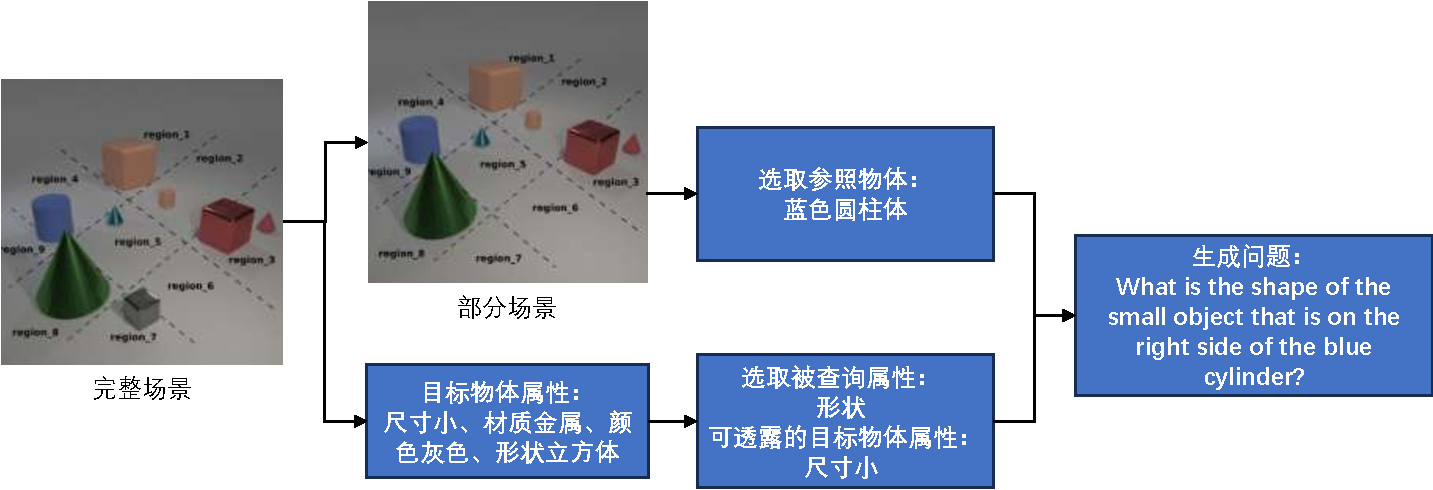
\includegraphics[scale=0.6]{figures/部分场景及问题生成-crop.pdf}
\caption{构建不可见场景图流程图}
\label{generate-partial-scenes-and-questions}
\end{figure}

选择目标物体的过程需要满足以下条件:
\begin{enumerate}[nosep]
\item 从完整场景图的所有物体中随机选取一个,在随机选取的过程中,要注意保持均衡,不能
一直选取单一区域的物体或者相同属性的物体,以免造成数据偏态分布。
\item 被选择物体不能是唯一出现某一属性的对象,避免由于移除该物体后,
导致场景图中该属性的值无法被推断,导致问题无解。
\item 该物体将在后续问题中作为查询目标。
\end{enumerate}

选择$Obj_i$后,需要将完整场景图中关于$Obj_i$的所有信息全部移除,生成部分场景。
从而得到一个只包含可见物体的子结构,记为 $Partial_i$,该场景图中缺少了目标物体的显式信息。
\end{enumerate}
\subsubsection{图像渲染}
图像渲染的目的是依据部分可见场景图以及不可见场景图,使用Blender进行渲染生成图像,生成最终完整的部分可见场景和不可见场景。本环节的具体步骤如下:
\begin{enumerate}[nosep]
\item 初始化Blender渲染对象。在这一步中,主要是设置一系列渲染参数,包括分辨率、GPU设置等等。
\item 定义场景字典。该字典中保存了场景的元信息(即将生成的图片名称等)、物体信息和方向信息。
\item 方向向量计算。先获取在场景初始化时添加的平面的法向量,此后计算摄像机的方向向量,并将
摄像机的方向向量投影到平面上,得到相对于平面的方向向量。计算完成之后,将平面删除,避免影响后续渲染
\item 向场景中添加物体。根据场景图中的物体信息,将物体添加到场景中。添加过程中,要注意确保物体之间的距离和边距满足约束条件。
此外,在生成部分可见场景时,要注意根据部分可见场景图中的遮挡物体和遮挡面积比例,来生成遮挡的情形;
在生成不可见场景时,要注意。
\item 计算物体之间关系。基于物体的三维坐标和场景的方向向量,遍历场景中的每对物体,
计算得出空间中上、下、左、右、前、后等关系。判断两个物体之间是否存在某种关系的阈值设置为0.2,即如果两个物体之间的
方向向量的点积大于0.2,那么认为它们具有该关系。
\end{enumerate}
最终,输出一个JSON对象,其中描述了场景中所有物体之间的空间关系,一个可能的字典如图所示,其中$left[0] = 1$说明
物体0的左侧有物体1,$right[1] = 0$说明物体1的右侧有物体0。
\begin{lstlisting}
{
    "left": [[1], [], [], []],
    "right": [[], [0], [], []],
    "above": [[], [], [3], []],
    "below": [[], [], [], [2]],
    "front": [[1], [], [], []],
    "behind": [[], [0], [], []]
}
\end{lstlisting}

在图像渲染完成之后,整个场景构造完成,此时进行数据整合,将所有场景文件合并同一个包含所有场景的JSON文件中。
\subsubsection{问题生成}
POVQAD根据前述步骤整合的场景文件和问题模板来构造自然语言问题,
一种供参考的模板如\ref{asp:question-template}中所示,
其中<Z1>、<Z2>均表示形状,<C1>、<C2>均表示颜色,<M1>、<M2>均表示材质,<S1>、<S2>均表示尺寸,
<R>表示空间关系。该模板旨在提问具有某种属性的两个物体之间是否处于某种空间位置关系。
这种模板化设计不仅使自然语言问题的结构化描述成为可能,
而且便于后续转换为ASP的形式化表示,从而实现问题求解的自动化。
本文设置了
\begin{lstlisting}[label=asp:question-template]
Is the <Z1> <C1> <M1> <S1> <R> the <Z2> <C2> <M2> <S2>?  
\end{lstlisting}

首先,筛选问题模板。对模板的筛选,按照模板的查询目标是否与当前场景相匹配,以及模板中给定信息是否在场景中存在来进行。

问题模板筛选完毕之后,根据场景图和筛选好的问题模板,进行模板实例化,生成问题文本及其对应的ASP查询。
实例化过程中,需要对模板中的占位符替换为具体的属性值。对每一个自然语言问题,都是从一个问题模板出发,填充占位符,
然后生成的。所以,自然语言和ASP查询具有一一对应的逻辑结构,可以实现自动转换。

此后调用Clingo求解查询,生成问题的答案,并通过对答案进行分析,实现对生成问题的筛选。
筛选逻辑是:如果答案集为空或者包含所有的可能值,则丢弃当前问题。对生成问题进行筛选有以下三点原因:
\begin{enumerate}[nosep]
\item 提高问题的质量。确保生成的问题有明确的答案,而不是模糊或无意义的问题。
\item 避免冗余问题。避免生成答案集过大的问题,这些问题可能对模型训练没有帮助。
\item 确保问题的多样性。筛选掉覆盖所有可能答案的情况,确保问题具有一定的区分性。
\end{enumerate}

最后,将生成的问题、ASP查询和答案保存为JSON文件,每个问题对应的积木世界图像的名称和序号也会一同记录。
\subsection{数据集质量评估}
为验证构造的POVQAD数据集的可靠性与研究价值,本节从POVQAD的可执行性与一致性、统计分析、对比实验方面进行研究。
\subsubsection{可执行性与一致性评估}
可执行性指的是POVQAD中每个样例的ASP程序能够经Clingo求解器执行,不出现语法错误。
一致性指的是对POVQAD中每个样例的ASP程序,Clingo对其的求解结果与样例中给出的标准答案一致。

本文对POVQAD中所有ASP程序依次使用Clingo进行执行,统计语法错误率,结果为0.2\%,
并且对能够正确执行的ASP程序的运行结果与标准答案进行对比分析,一致率为99.5\%,以上两点证明本文生成的ASP程序质量较高,
使用ASP构造POVQAD的方法合理。
\subsubsection{统计分析}
POVQAD中问题分布的统计图见\ref{fig:question_statistics},从图中可以看到位置类问题占比34\%,位置关系类问题占比33\%,
与位置有关的计数类问题占比33\%,总体上实现了三类问题占比1:1:1的要求,做到了问题类型的均匀分布,
这样设计一方面有助于全面评估模型在不同空间推理任务中的能力,避免模型对某一类型问题的过拟合;
另一方面也提升了数据集的科学性和可解释性,使得模型性能对比更加公平合理。
此外,均衡的问题分布也为后续在不同子任务上的研究提供了良好的数据支持基础。
\begin{figure}[h]
    \centering
    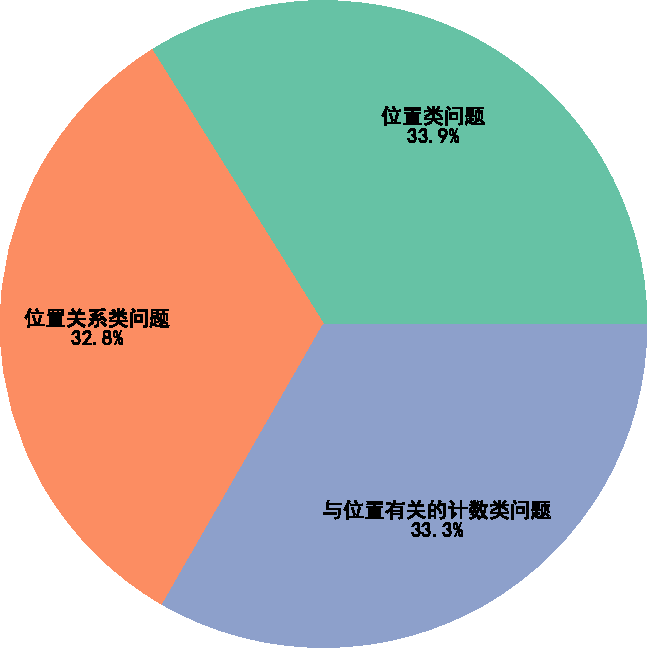
\includegraphics[scale=0.6]{figures/三种类型问题占比-crop.pdf}
    \caption{问题类型分布}
    \label{fig:question_statistics}
\end{figure}
\subsubsection{对比实验}
为了证明POVQAD数据集对不同推理能力方法的区分性与挑战性,
本文选取了五种代表性方法在该数据集上进行实验:传统感知模型(CNN+LSTM)、
主流多模态大模型(DeepSeek、Gemini 2.5 Flash、ChatGPT-4o),以及人类作答作为理论上限参考。
每种方法的输入为POVQAD的图像、自然语言问题以及环境约束。实验重复进行三次取平均值,最终实验结果如图\ref{fig:dataset-comparison}所示,可得出如下结论:
\begin{enumerate}[nosep]
\item 数据集具有良好的难度区分能力。各方法在POVQAD上的准确率差异明显,充分体现了模型间的空间理解与逻辑推理能力差距。尤其是传统模型(CNN+LSTM)仅达到 45.4\% 的准确率,明显低于VLMs方法,显示POVQAD对浅层感知模型构成了挑战。
\item 多模态大模型在不完全信息推理方面存在性能瓶颈。
即便是先进的多模态大模型(如 ChatGPT-4o)也未能达到人类水平,
在复杂场景、信息遮挡和规则约束下的准确率仍有明显提升空间,说明POVQAD能有效考察模型对隐含信息与环境规则的建模能力。
\item POVQAD能作为更强推理任务的评估基准。
结果表明,POVQAD能有效区分浅层感知模型与具备显式推理机制的方法,
同时能检测当前主流多模态模型在空间推理与知识补全方面的能力边界,具备良好的基准测试价值。
\end{enumerate}
\begin{figure}[h]
\centering
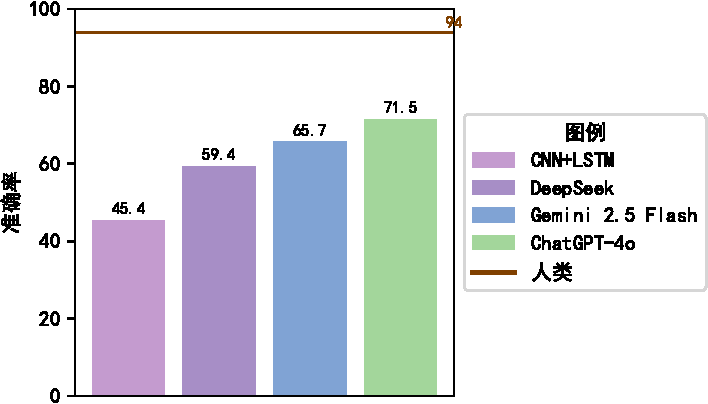
\includegraphics[scale=0.8]{figures/dataset-experiment-crop.pdf}
\caption{不同方法在POVQAD上回答问题的准确率}
\label{fig:dataset-comparison}
\end{figure}
\section{本章小结}
本章聚焦CLEVR数据集的场景完全可见、不要求模型使用外部背景知识进行推理等方面的缺陷,构建一个新的数据集POVQAD,以满足
本文对部分可见积木世界场景下空间推理问答的研究需要。

本章为后续神经符号VQA框架在部分可见积木世界场景下的空间推理问答的实验与分析奠定了坚实的数据基础。